\documentclass[border=2pt]{standalone}
\usepackage{tikz}
\usetikzlibrary{shapes,arrows,positioning}
\begin{document}
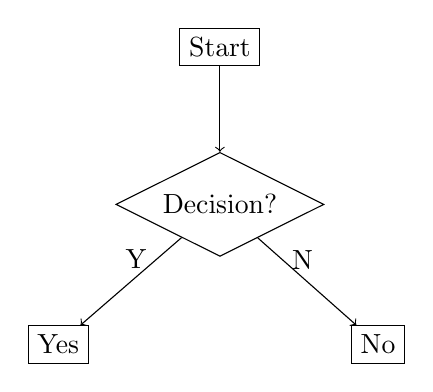
\begin{tikzpicture}[node distance=2cm, auto]
  \node[rectangle, draw] (start) {Start};
  \node[diamond, draw, below of=start, aspect=2] (decision) {Decision?};
  \node[rectangle, draw, below left=1.2cm and 1cm of decision] (yes) {Yes};
  \node[rectangle, draw, below right=1.2cm and 1cm of decision] (no) {No};
  \draw[->] (start) -- (decision);
  \draw[->] (decision) -- node[near start, left] {Y} (yes);
  \draw[->] (decision) -- node[near start, right] {N} (no);
\end{tikzpicture}
\end{document}
